\begin{corrige}{CourbesSurfaces0004}

La fonction $x$ est définie pour toute valeur de $t$, mais $y$ n'est pas définie en $t=0$. Notre courbe sera alors l'union de deux branches, la première définie pour $t>0$ et l'autre pour $t<0$. On remarque tout de suite que les limites de $x$ et $y$ lorsque $t\to 0^{\pm}$ sont, respectivement, $0^\pm$ et $+\infty$ (la courbe ressemble à $(2t, 1/t^2)$). Par contre, lorsque $t\to \pm\infty$ on a $x\to +\infty$ et $y\to 0^\pm$ (la courbe ressemble à $(t^2, 2/t)$). 

Ni $x$ ni $y$ ont des symétries remarquables. 

On cherche tout de suite les intersections avec les axes : $x(t)=0$ pour $t=0$ et $t=-2$. Comme $t=0$ ne fait pas partie du domaine la seule intersection avec l'axe verticale est $(0, y(-2)=-3/4)$. Le seul zéro de $y$ est $t=-1/2$, l'intersection avec l'axe horizontale correspondante est $(x(-1/2)=-3/4,0)$. 

Les dérivées de $x$ et de $y$ sont $\dot x (t)= 2t+2 $ et $\dot y(t)= -2/t^3-2/t^2$. Le point $t=-1$ est donc un point critique pour les deux fonctions. Plus précisément, il s'agit d'un minimum pour $x$ et $y$ : $x(-1)=-1$, $y(-1)= -1$.

 Il faut bien comprendre qu'il s'agit  d'un minimum pour la branche qui correspond à  $t<0$ mais que pour $t>0$ $y$ pourrait bien prendre des valeurs encore plus petits. Pourriez vous dire pourquoi cela ne peut pas arriver à $x$ ? On peut voir un exemple de ce comportement dans le deuxième exercice de ce devoir.   
Nous pouvons observer que pour $t>0$ $x$ est strictement croissante et $y$ strictement décroissante. 

Les deux branches de cette courbe sont tracées dans la figure \ref{figdevoir3exo1}.

\begin{figure}
  \begin{center}
    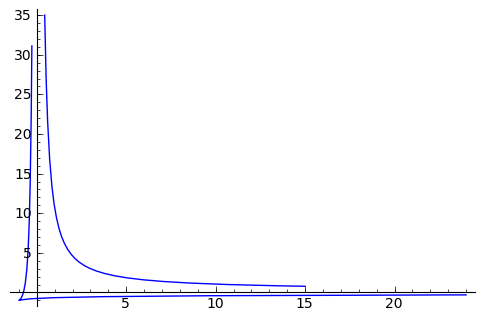
\includegraphics[width=9cm]{figdevoir3exo1.png}

  \caption{La courbe de l'exercice \ref{exoCourbesSurfaces0004}}\label{figdevoir3exo1}
  \end{center}
 \end{figure}
\end{corrige}
